
Com o intuito de avaliar o comportamento das diferentes implementações de código aberto de núcleo 5G para execução dos procedimentos em escala e utilizando-se como base a prova de conceito do trabalho de \cite{Dominato2021}, foi desenvolvida uma extensão para a aplicação \textit{my5G-RANTester}\footnote{https://github.com/my5G/my5G-RANTester}.
Esse projeto implementa um testador que tem como objetivo simular e realizar testes sobre os planos de controle e de dados de um equipamento de usuário e de uma estação de rádio base da rede 5G.
O testador foi projetado para realizar testes de conformidade e robustez sobre diferentes implementações de código aberto de núcleos de redes 5G, todavia o testador suporta a expansão para outras cargas de trabalhos, permitindo o desenvolvimento de outros tipos de testes, como testes de desempenho que estão sendo abordados nesse trabalho de graduação.

Uma arquitetura em alto nível da aplicação desenvolvida pode ser vista na Figura \ref{fig:tester_arch}.
A prova de conceito implementa as camadas de Simulação, do Controlador e da Interface de usuário.
A implementação que foi utilizada como base é feita na linguagem de programação \textit{Go}, criada pela Google em 2009\footnote{https://go.dev/}.

A camada de Simulação simula o comportamento de uma ou mais gNodeB e de um ou mais equipamentos de usuário.
Nessa camada, a diferença entre a implementação feita no trabalho de \cite{Dominato2021} e o que foi feito no presente trabalho é a capacidade de simular múltiplas gNodeB e UEs simultaneamente, com o intuito de validar a performance de cada implementação de núcleo da rede.

A camada do Controlador é a principal camada no funcionamento do testador. Essa camada recebe os comandos do usuário através de uma interface que define qual teste será executado, controla a camada acima e faz a coleta das métricas do experimento.
Os planos de testes representam os testes em si que foram escolhidos para serem executados. O Executor recebe as informações do teste e configura as gNodeB e os UEs e envia as métricas para o Coletor de métricas, que irá armazená-las para futuros usos.

Por fim, a camada da Interface de usuário permite a execução e o monitoramento dos testes, além de exportar as métricas armazenadas na camada acima. É com essa camada que o usuário do testador pode interagir através de parâmetros enviados por uma linha de comandos a ser executada no ambiente de testes.


\begin{figure}[!ht]
    \centering
    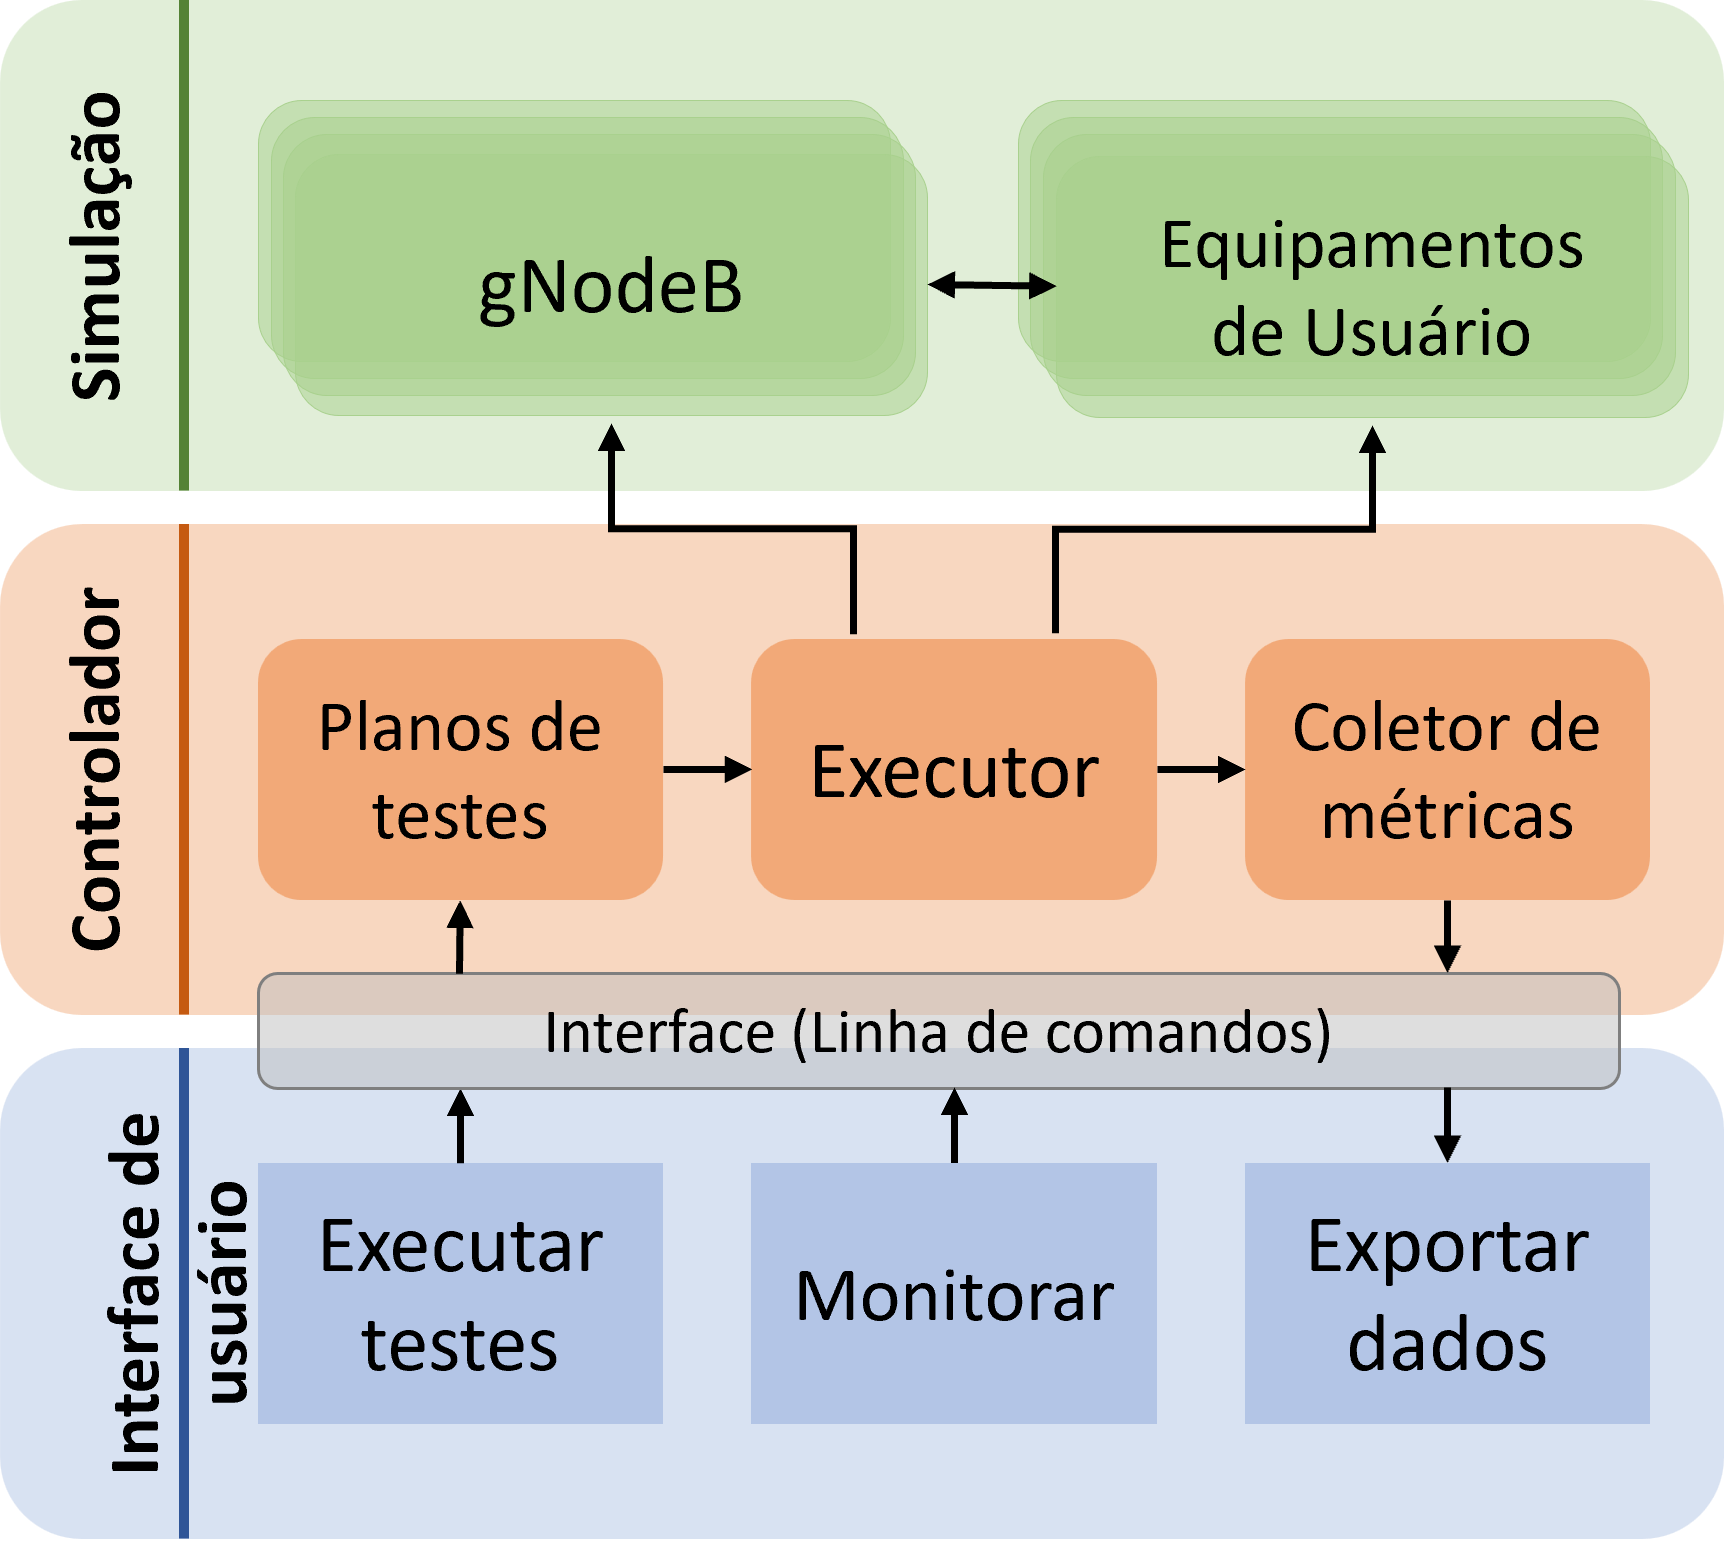
\includegraphics[width=0.6\textwidth]{TG2/Chapters/Soluction/Figures/Arquitetura-Componentes.png}
    \caption{Arquitetura do testador}
    \label{fig:tester_arch}
\end{figure}


\textcolor{red}{Escrever um parágrafo explicado quais itens serão explicados a seguir.}

\subsection{Módulo de teste}

Para a execução de testes de desempenho, foi desenvolvido um módulo para o testador que permite a execução de múltiplas conexões de equipamentos de usuários simultâneas.
Esse módulo possui parâmetros de configuração para facilitar variações entre os testes. Os parâmetros suportados são o número de equipamentos de usuário a ser conectados, o atraso em milissegundos entre uma conexão e outra e o atraso em segundos para começar a execução do experimento.

No começo da execução, esse módulo simula uma gNodeB e inicia a conexão com o núcleo da rede. Após a conexão ser bem sucedida, é aguardado o tempo para iniciar a execução do experimento.
Ao iniciar o experimento, o módulo inicia um fluxo de trabalho em paralelo para criar uma nova instância de equipamento de usuário e realizar a conexão com o núcleo da rede.
Após iniciar o fluxo de trabalho em paralelo, o módulo aguarda o atraso entre conexões definido pelo usuário antes de iniciar o próximo fluxo, até que a quantidade de dispositivos definida pelo usuário seja atingida.

Devido a uma limitação do testador, que não consegue gerenciar mais de 255 equipamentos de usuário simultaneamente, foi decidido criar múltiplas instâncias do testador, cada uma simulando uma gNodeB diferente, todas se conectando no mesmo núcleo.
Sendo assim, foi possível testar o comportamento de um núcleo de rede 5G com múltiplos equipamentos de usuário e estações de rádio base.

Com o objetivo de realizar todas as execuções dos experimentos o mais similares possível, foi desenvolvido um orquestrador, que gerencia toda a execução do experimento, como será explicado com mais detalhes adiante.

\subsection{Módulo de coleta de dados do testador}

Para realizar a coleta de dados, foi desenvolvido um módulo de coleta das métricas dos equipamentos de usuário, visto que o testador não possuía suporte para essa funcionalidade até o momento que esse trabalho de graduação foi desenvolvido.

O módulo de coleta de métricas consiste em um fluxo de execução em paralelo que registra o tempo (em nanossegundos) que cada equipamento de usuário demorou para trocar entre cada estado da conexão com o núcleo da rede 5G.
As informações de tempo para cada estado de cada equipamento de usuário são escritas na saída de texto padrão do contêiner utilizado pela instância do testador.

Ao final da execução, uma aplicação foi desenvolvida para realizar o processamento dos registros gerados através das diversas instâncias do testador, fazendo um pré processamento dos dados, ordenando eles com base no horário da inicialização do equipamento de usuário (em nanossegundos a partir do \textit{epoch time}) e gerando um arquivo de texto separado por vírgulas, permitindo a fácil importação dos resultados através de programas de análise de dados.
Inicialmente, essa aplicação foi desenvolvida para coletar e processar os registros de uma única instância do testador, ordenando os dados no arquivo de saída em ordem crescente do identificador do equipamento de usuário. Entretanto, foi necessário modificar essa aplicação para suportar múltiplas instâncias de testadores e reordenar os dados do arquivo de saída, visto que a ordem de conexão dos dispositivos deixou de ser realizada em ordem crescente do identificador.

\subsection{Módulo de coleta de dados do núcleo}

O desenvolvimento deste módulo teve a contribuição do bolsista de iniciação científica do projeto Porvir.
Esse módulo consiste na implementação de um fluxo sobre uma instância da aplicação \textit{Node-RED}\footnote{https://nodered.org/}.

Um fluxo foi desenvolvido para listar todos os contêineres em execução na máquina e realizar a coleta das métricas do \textit{Docker} e armazená-las em uma instância do banco de dados \textit{InfluxDB}\footnote{https://www.influxdata.com/}. Esse fluxo foi definido para ser executado automaticamente após a inicialização do contêiner do \textit{Node-RED}, permitindo a coleta de dados de uso de disco, rede, processador, memória, entre outras, de forma automatizada pelo orquestrador do experimento.

\subsection{Orquestrador}
\label{sub:arch-orchestrator}

O orquestrador consiste em uma série de roteiros de execução, desenvolvidos em sua maioria sobre as linguagens \textit{Bash Script} e \textit{JavaScript}.
A Figura \textcolor{red}{A FAZER} representa um diagrama de blocos do fluxo de execução do orquestrador.
O orquestrador é executado através de uma interface de usuário por linha de comandos, suportando diversos comandos para definir os parâmetros de execução do experimento, permitindo ao usuário automatizar a execução de experimentos de forma simplificada.

Os parâmetros suportados são a quantidade total de equipamentos de usuário a serem conectados no núcleo da rede, a quantidade de testadores que serão executados em paralelo, o tempo em milissegundos para ser aguardado entre cada conexão de equipamento de usuário, o tempo em segundos para aguardar a inicialização e qual núcleo da rede 5G deve ser utilizado pra executar o experimento.
Além dos parâmetros de execução do experimento, o orquestrador também permite o usuário interromper a última execução e limpar o ambiente de testes, removendo todos os contêineres e dados gerados pelo experimento, além de permitir executar o orquestrador em modo de depuração, exibindo para o usuário todos os registros de execução.

\textcolor{green}{Desenho com a lógica dos blocos}

\textcolor{red}{No bloco de instanciar o core, foi criado um código para cada core.}

\textcolor{red}{Script do FGCore em apêndice?}

\textcolor{red}{Tem duas versões e será feita uma terceira para ser executada em cada core. Falta o do oai.}